Linebacker 2

DESIGNER: Claes Henrikson
Graphics: Fredrik P. Malmberg
Copyight ©1979
Swedish Game Production

\section*{INTRODUCTION}
LINEBACKER 2 is a strategic game
of the bombing of North Viet Nam in
late 1972.

\section*{SETTING UP THE GAME}
First, see scenario instructions for
information on the forces available
to each player. The North Vietnamese
(NV) player divides his fighter unit
counters between his air bases on his
air status display. Two units (four
planes) may begin the game in the
air, represented on the game map by
its proper echo marker (see move-
ment). He then proceeds to indicate
the number of available Anti-Aircraft
missiles on his SAM SUPPLY TABLE.
The United States (US) player
divides his available air units between
the target boxes on his air status
display and places the corresponding
echo counters face-down in the US
holding area on the game map.

%  Define a macro for inserting the graphic
\newcommand{\bfiftytwo}{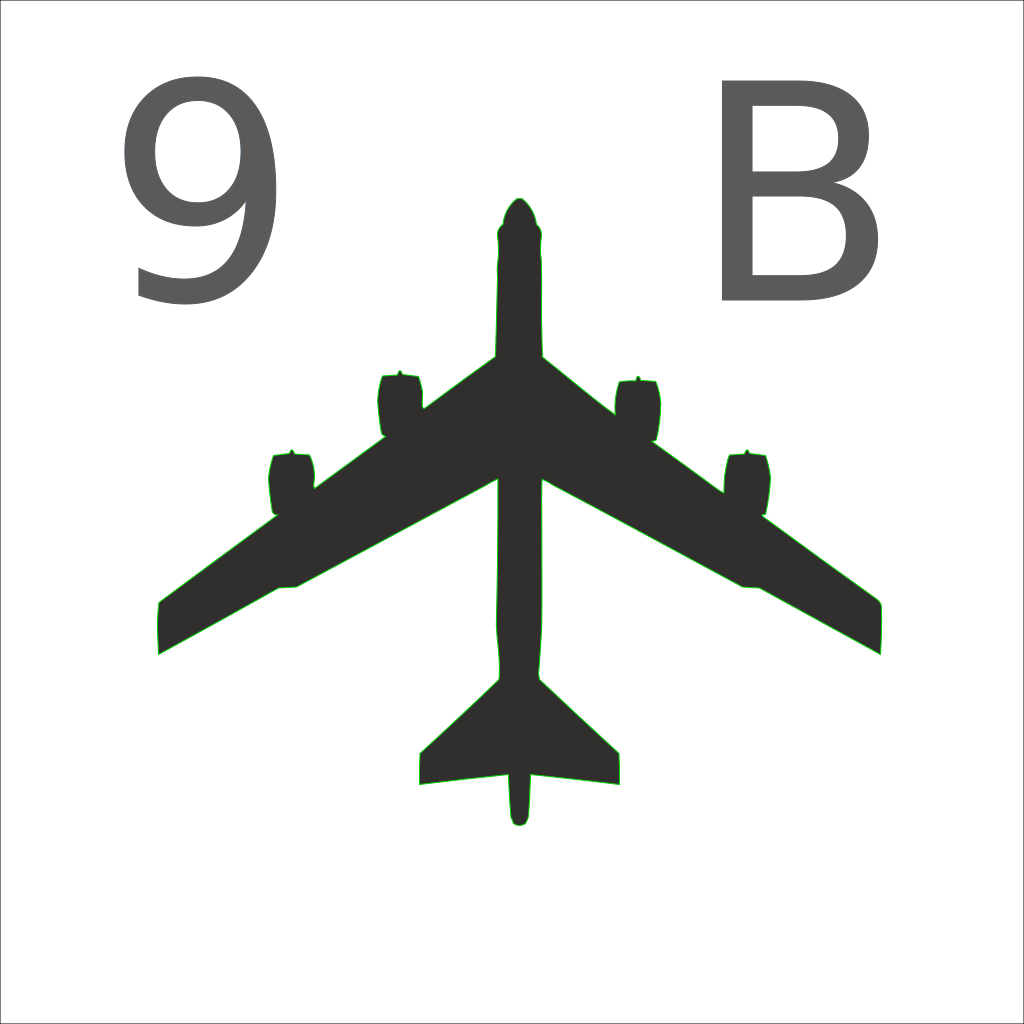
\includegraphics[width=0.25in]{../counters/b52-counter.pdf}}
\newcommand{\ffour}{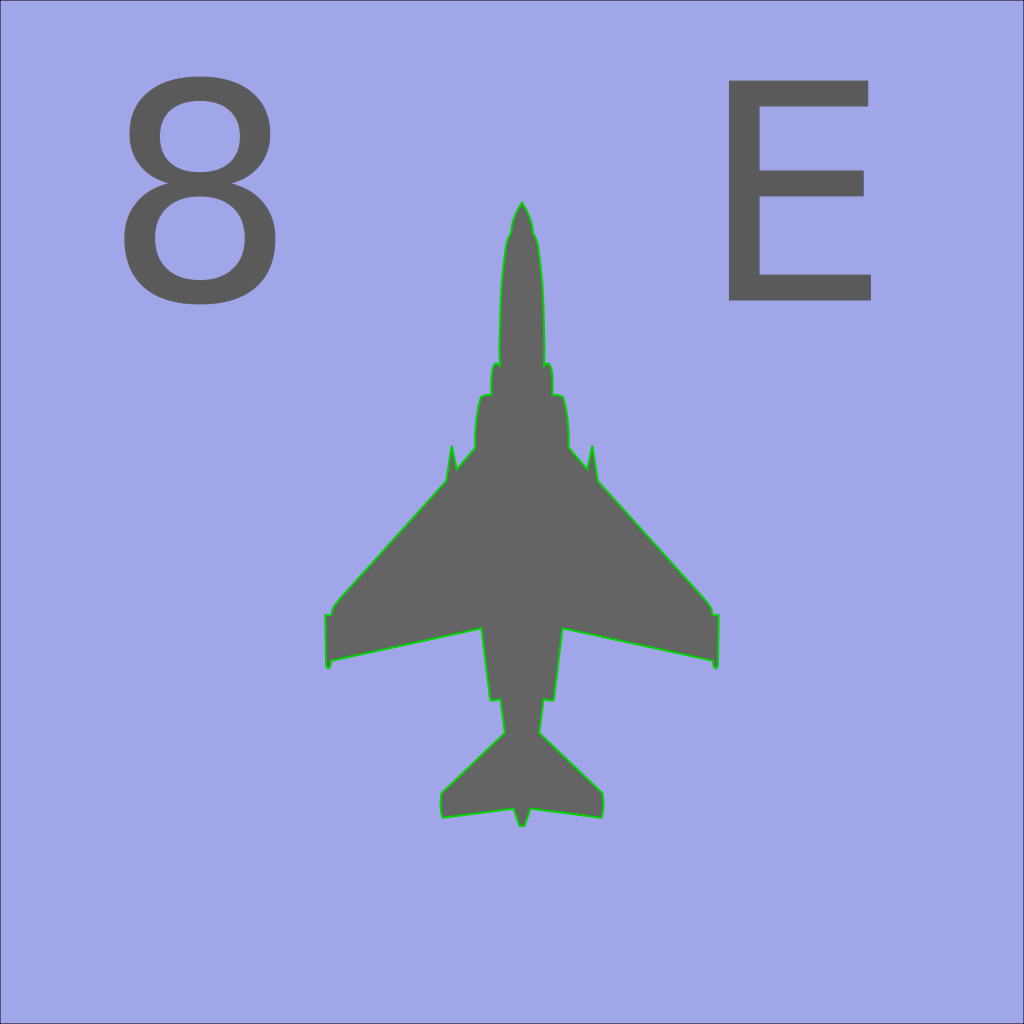
\includegraphics[width=0.25in]{../counters/f4-counter.pdf}}
\newcommand{\foneeleven}{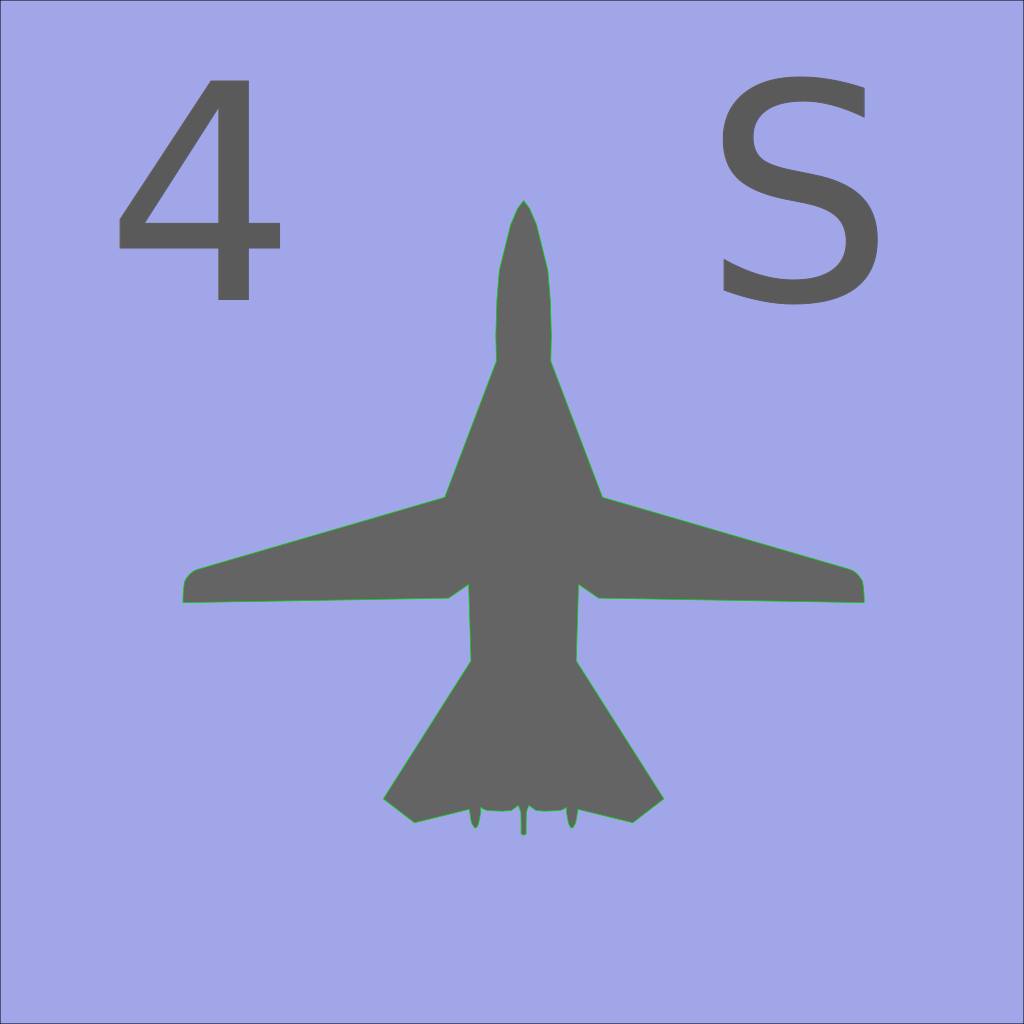
\includegraphics[width=0.25in]{../counters/f111-counter.pdf}}
\newcommand{\plus}{
\includegraphics[width=0.25in]{../counters/plus-counter.pdf}}
\newcommand{\migtwoone}{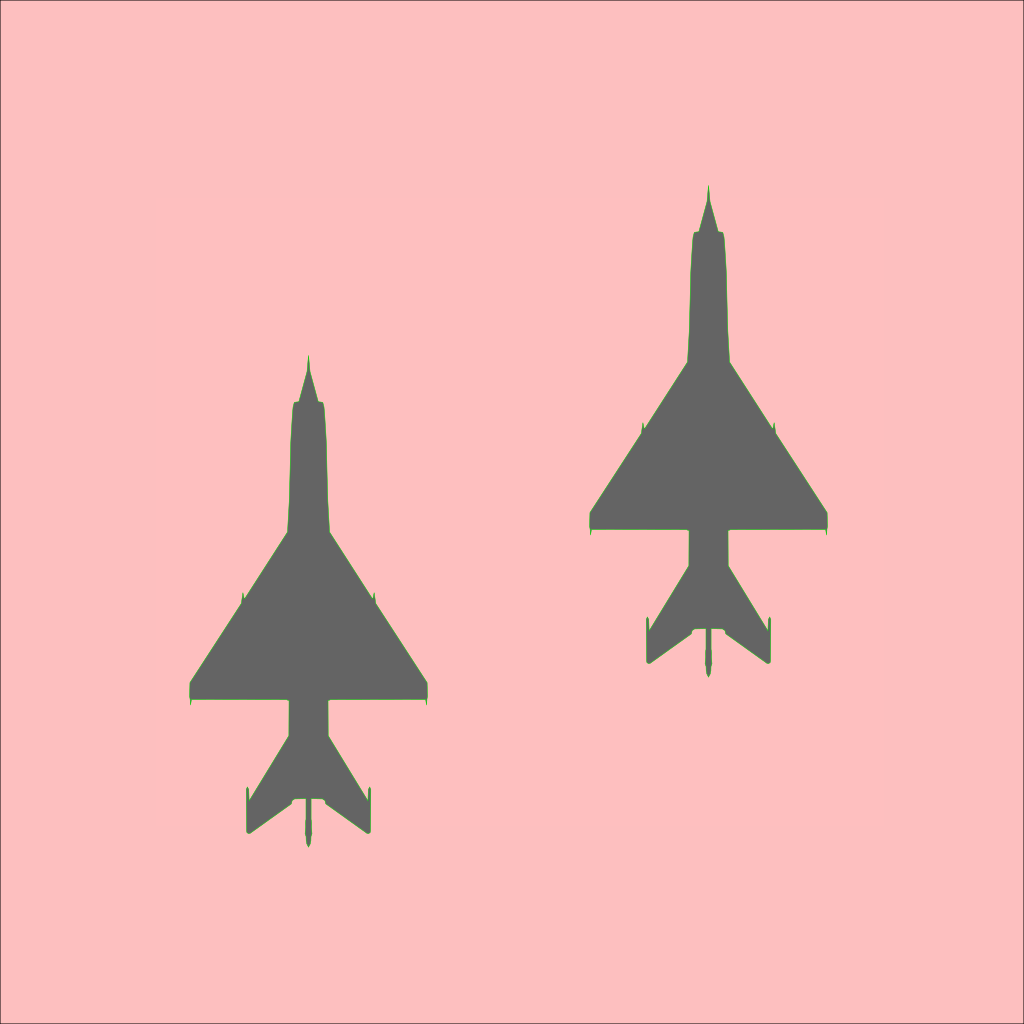
\includegraphics[width=0.25in]{../counters/mig21-counter.pdf}}
\newcommand{\radar}{
\includegraphics[width=0.25in]{../counters/radar-counter.pdf}}
\newcommand{\hit}{
\includegraphics[width=0.25in]{../counters/hit-counter.pdf}}
\newcommand{\sam}{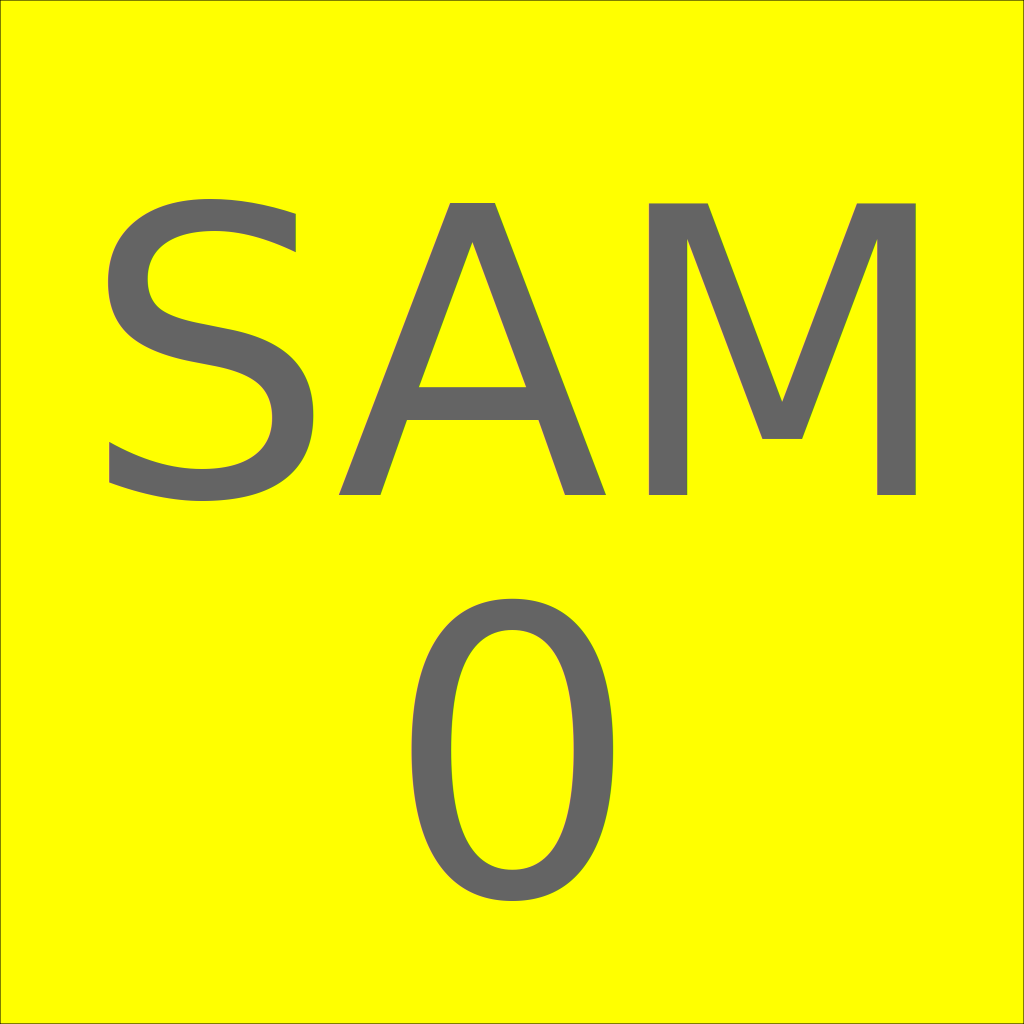
\includegraphics[width=0.25in]{../counters/sam-counter.pdf}}

\section*{UNITS}
\noindent
\begin{tabularx}{\linewidth}{@{} m{0.3in} X @{}}
   \radar & Radar Echo \# - confirms to MISSION DISPLAY \#indicator \\
   \bfiftytwo & 3 B-52 bombers \\
   \foneeleven & 4 F-111 strike aircraft \\
   \ffour & 8 F-4 strike fighters/escort fighters \\
   \plus & 1 A-6 EMC aircraft \\
\end{tabularx}

\noindent
\begin{tabularx}{\linewidth}{@{} m{0.3in} X @{}}
   \hit & 1 aircraft downed \\
   \migtwoone & 2 MiG-21 fighters \\
   \sam & SAM supply indicator [hundreds, tens, and ones] \\
 \end{tabularx}

 %%% TODO: Change subitem heading to A, B, C, etc.
\section*{SEQUENCE OF PLAY}
\begin{enumerate}[nosep]
    \item First SAM fire phase
    \item Air-to-Air combat phase:
        \begin{enumerate}[nosep]
            \item Interception segment
            \item B-52 defensive fire segment
            \item Air superiority segment
        \end{enumerate}
    \item Bombing phase:
        \begin{enumerate}[nosep]
            \item Low-level flak attack segment
            \item Bombing phase
        \end{enumerate}
    \item Movement phase:
        \begin{enumerate}[nosep]
            \item First player movement segment
            \item Second player movement segment
        \end{enumerate}
    \item Second SAM fire phase
    \item Record the passage of one GAME TURN
\end{enumerate}


Each game turn is divided into
several phases. Follow the above
sequence every game turn performing
actions as per the rules given for each
phase.

\section*{SAM FIRE}
All SAM fire takes place during the
two SAM FIRE PHASES. The NV
player may fire SAMs at all, any or
none of the US echo counters in a map
box (except the US HOLDING AREA
Box). He decides the number of SAMs
fired in each salvo and resolves
combat on the proper column of the
FLAK CRT, subtracting the number
of fired SAMs on the SAM SUPPLY
TABLE.

An echo counter may only be fired
at once in every SAM Fire Phase.
